%% Source of figures/sample-plot.pdf
%% Rebuild with:  pdflatex sample-plot.tex && mv sample-plot.pdf ..
\documentclass[border=2pt]{standalone}
\usepackage[T1]{fontenc}
\usepackage{mathpazo}
\usepackage[scaled=0.92]{helvet}
\usepackage{tikz}
\definecolor{accent}{HTML}{1F4E79}
\definecolor{second}{HTML}{B45309}
\begin{document}
\sffamily\small
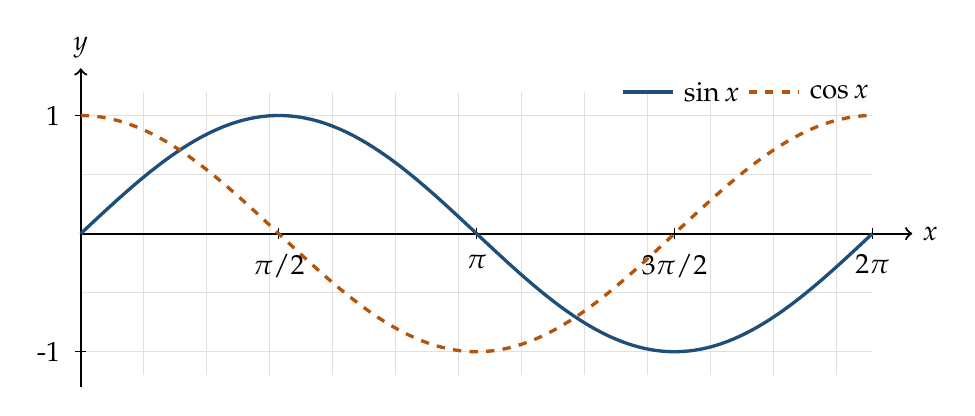
\begin{tikzpicture}[x=1.6cm,y=1.5cm]
  % grid and axes
  \draw[black!12] (0,-1.2) grid[xstep=0.5,ystep=0.5] (6.28,1.2);
  \draw[->,thick] (0,0) -- (6.6,0) node[right] {$x$};
  \draw[->,thick] (0,-1.3) -- (0,1.4) node[above] {$y$};
  \foreach \x/\l in {1.571/{$\pi/2$},3.142/{$\pi$},4.712/{$3\pi/2$},6.283/{$2\pi$}}
    \draw (\x,2pt) -- (\x,-2pt) node[below=2pt] {\l};
  \foreach \y in {-1,1} \draw (2pt,\y) -- (-2pt,\y) node[left=2pt] {\y};
  % curves
  \draw[accent,very thick,domain=0:6.283,samples=80,smooth] plot (\x,{sin(\x r)});
  \draw[second,very thick,dashed,domain=0:6.283,samples=80,smooth] plot (\x,{cos(\x r)});
  % legend
  \draw[accent,very thick] (4.3,1.2) -- ++(0.4,0) node[right,black] {$\sin x$};
  \draw[second,very thick,dashed] (5.3,1.2) -- ++(0.4,0) node[right,black] {$\cos x$};
\end{tikzpicture}
\end{document}
